\ifx\wholebook\relax\else
\input{../Common.tex}
\input{../macroes.tex}
\begin{document}
\fi

\chapter{Methods: Named Message Sequences}\label{ch:turtleTeaching}\label{ch:abstraction}\label{cha:enseigner}

%\begin{chapterfigure}
%
\includegraphics[width=0.9\linewidth]{carosName}
%\end{chapterfigure}

%\begin{figure}
%\center{\includegraphics{microBrowserInWorking}}
%\caption{ .\label{fig:microBrowserInWorking}}
%\end{figure}


Up to now, you used scripts: you created first a robot and sent a sequence of 
messages to it. Using scripts is a straightforward approach, but it has some 
severe limitations. One of the major limitation is that a script cannot be called by another script. This is a real problem because a script cannot be reused by other scripts. Moreover you cannot decompose a complex problem into simpler problems and then recompose them to solve the complex problem.

Wouldn't it be nice if one could define a kind of script whose sequence of messages could be sent to any robot. Well, this is of course possible and such a sequence of messages is called a \emph{method}\footnote{In the context of this book we will not elaborate on the real power of methods as this has to do with 
object-oriented programming.}. A \emph{method} is a named sequence of messages. This name can be used in a script or even in another method.  In fact, all robot messages used so far are methods that you used on any robot. 

In this chapter, you shall learn how to define methods. You already know most of the things needed to write the code of the methods. However method must be defined using  a special editor called \index{code browser} \index{browser} a code browser. We start by comparing a script and a method. Then we will define a method then finally step back and really look in detail at what we did.


\section{Scripts versus Methods}
Let us look at one of the scripts you have been written so far, for
example, the script~\ref{src:againSquare} that created a
robot and asked it to draw a 100 pixels width square. 

\begin{scriptwithtitle}{A simple square}\label{src:againSquare}
| \caro |
\caro := \Turtle new.
4 timesRepeat: 
   [ \caro turnLeft: 90.
   \caro go: 100 ]
\end{scriptwithtitle}

The problem with a script is that each time you need to draw a square
you need to \emph{copy} the 3 last lines of \scriptref{src:againSquare}.  In addition, if you want that the square be drawn by another robot, \daly for example, you must change everywhere the name \caro to \daly. This is illustrated by \scriptref{src:againSquare2}.

\begin{scriptwithtitle}{Two simple squares}\label{src:againSquare2}
| \caro \daly |
\caro := \Turtle new.
\daly := \Turtle new.
\daly jump: 200.
\daly color: Color red.
\textbf{
4 timesRepeat: 
         [ \caro turnLeft: 90.
         \caro go: 100 ].

4 timesRepeat: 
         [ \daly turnLeft: 90.
         \daly go: 100 ].}
\end{scriptwithtitle}

Because of all this, working with scripts is not easy. In
fact, we are quite convinced that the two following statements
reflect you personal experience with scripts.

\begin{itemize}
\item Writing long scripts is a painful task.

\item Repeating long scripts is boring and error prone. 

\item When copying complex scripts, the likelihood of making a
programming\footnote{As opposed to a syntax error, which would be
caught quickly by the computer. \emph{Programming} errors, on the
contrary, are quite difficult to catch.}  error, such as omitting a
line, is high.
\end{itemize}


In fact, we would like to \emph{define once and only once} a sequence of messages, to give it a \emph{name} and to be able to \emph{send it as message to any} robots just as any predefined robot messages such as \go, \north, \jump... 
         
With such an approach we define a new \emph{method} \ct{square}, and 
we can write the \scriptref{src:againSquareMethod} --- Do not yet execute it 
since the method \ct{square} has not yet been defined. What you see is that we 
do not have to duplicate and adapt the sequence of messages defining a square. We just use it twice. Now you should be convinced that defining method is worth the effort. 
   
\begin{scriptwithtitle}{Using the method \ct{square}}\label{src:againSquareMethod}
| \caro \daly | 
\caro := \Turtle new.  
\daly := \Turtle new.  
\daly go: 200.  
\daly color: Color red.
\textbf{\caro square.
\daly square}
\end{scriptwithtitle}


%%%%%%%%%%%%%%%%%%%%%%%%%%%%%%%%%%%%%%%%%%%%%%%%%%%
\section{How to Define a Method?}
In this section we give a cookbook recipe on how to create a method. 
As in the context of this book you will only define methods for the robots, we programmed some simple and dedicated code browsers (\ie tools to define methods) that will let you define methods for your robots. By default you get one \tb in the working flap, but you can always create one by grabbing its thumbnail from the dark blue flap. 
   
Using a \tb to define a method requires to (1) choose or create a method
category \ie a kind of method folder (Section~\ref{sec:createCategory}), (2) type the method and (3) then compile it (Section~\ref{sec:definingmethod}). Let us detail the different parts of a \tb.

\subsection{A \tb}
As we already said, defining methods requires to use a new editor shown in Figure~\ref{fig:methodEditor}. This browser is actually a simplified version of the browser used by \st programmers. 

\begin{figure}
\centerline{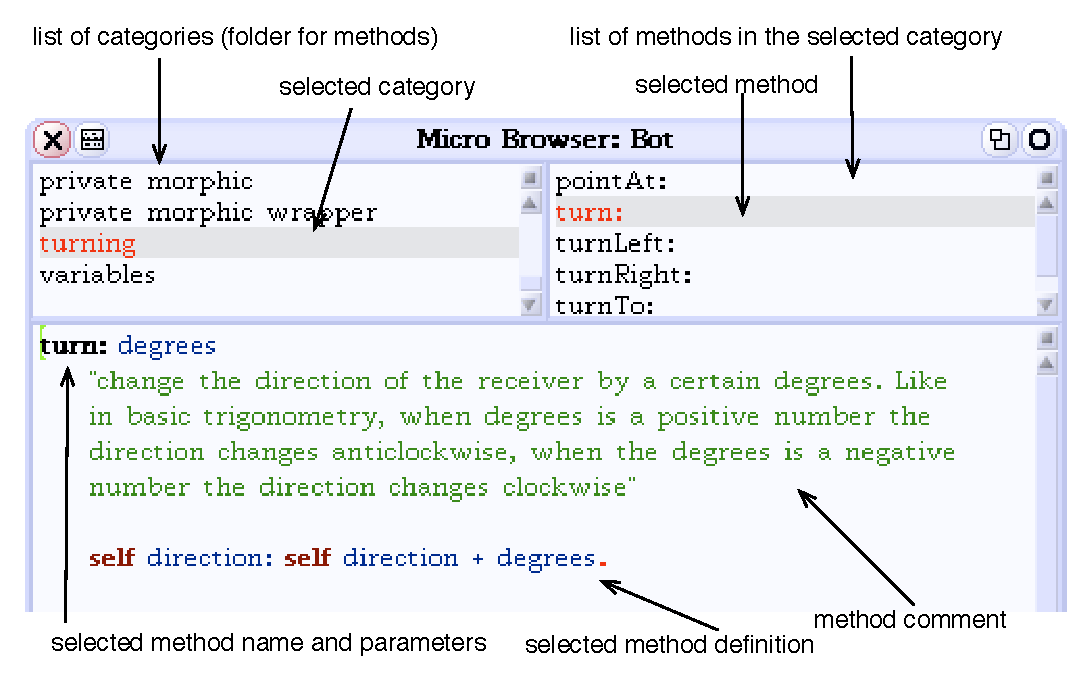
\includegraphics[width=10cm]{tbOneAnnotated}} 
\caption{The \tb showing the definition (bottom pane) of the 
method \ct{turn:} (right pane) belonging to the category \emph{turning} (left pane).\label{fig:methodEditor}}
\end{figure}

The browser consists of 3 parts:
\begin{description}
\item[Categories.] The left top part is the \emph{category list}.
It contains the method categories. Method categories are just names
that help us to group methods together so that we can find information
faster. In Figure~\ref{fig:methodEditor}, the category 'turning'
grouping all the operations having to deal with robot direction
changes is selected. Other categories grouping other robot behavior are listed.

\item[Methods.] The right top part is the \emph{method list}.
It contains the method names of the methods contained in the selected category. In Figure~\ref{fig:methodEditor}, five  methods are listed: \ct{pointAt:}, \ct{turn:} and \turnLeft, \turnRight, and \ct{turnTo:}. The method named \ct{turn:} is currently selected.

\item[Method Definition.] The bottom part is the \emph{code editor}. It shows the definition of the method whose name is selected. This is also the place where you can type the code of a new method.
\end{description}


\subsection{Creating a New Method Category}\label{sec:createCategory} 
Methods are grouped by categories. A category is simply defined by a name. To start defining a method, you must first define its category or select a category in which you want to define your method. Let us create a new category named regular shapes.

\begin{figure}
\centerline{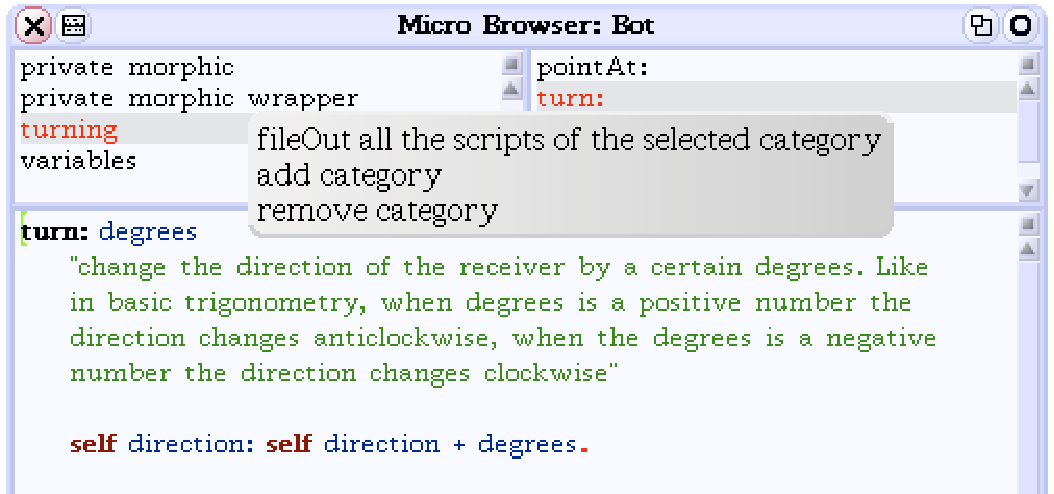
\includegraphics[width=10cm]{tbTwo}} 
\caption{To create a method category, in the category menu, select 'add category'.\label{fig:categoryMenu}}
\end{figure}
\begin{figure}\label{fig:categoryPrompt}
\centerline{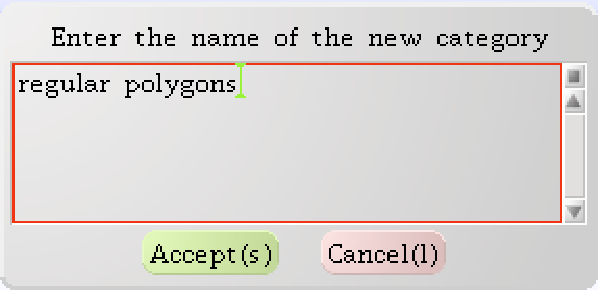
\includegraphics[width=6cm]{tbThree}}
 \caption{Entering the new category name.}
\end{figure}

\begin{enumerate}
\item Click with the right mouse button on the category list.
A menu such as the one of Figure~\ref{fig:categoryMenu} will show up.

\item Select the option \ct{add category} of that menu.

\item Type the name of the category in the dialog that pops up 
as shown in Figure~\ref{fig:categoryPrompt}.You may choose any name for the category. Of course, meaningful names are better if you want to share your work with other people or find
your way quickly. 

\item Click into the \ct{Accept} button to validate your  choice.
\end{enumerate}


As shown in Figure~\ref{fig:categorycreated} the name of the
new category appears in the category pane and is automatically
selected. The editor is ready to accept the new method definition. It shows 
you a reminder for the definition of method that you can remove when you start 
typing your method. You are now ready to define your first method.

\begin{figure}
\centerline{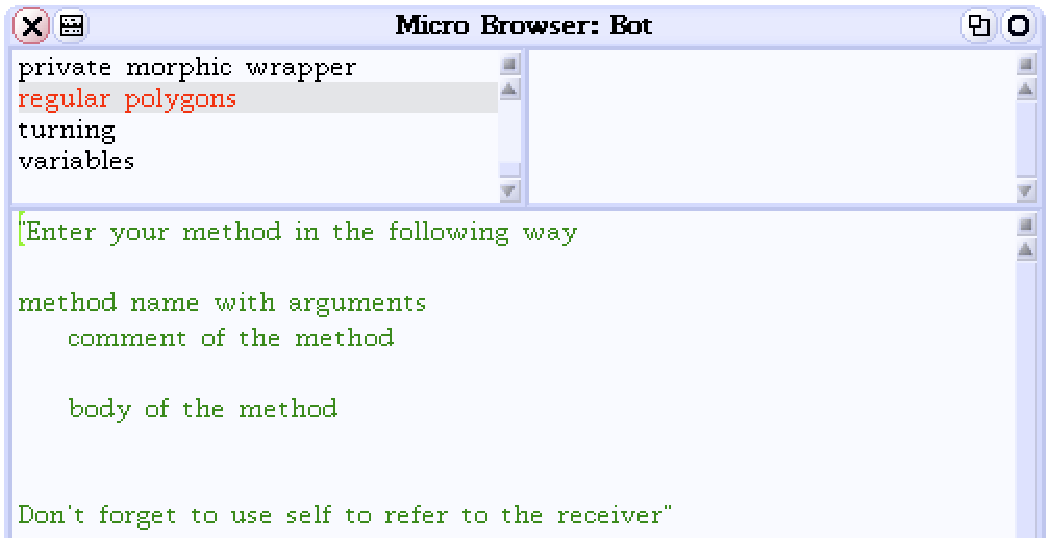
\includegraphics[width=10cm]{tbFour}}
\caption{The resulting category is created.\label{fig:categorycreated}}
\end{figure}

\subsection{Defining your First Method}\label{sec:definingmethod}
If the category in which you want to add your method is not selected,
select it. Then type in the method as shown by \methodref{mth:square}
shown below into the code editor pane. For that you can simply select the 
previous text and start typing your method. 

\begin{method}\label{mth:square}
square 
   "Draw a square of 100 pixel size"

   4 timesRepeat: 
                [ self go: 100.
                self turnLeft: 90 ]
\end{method}

Defining a method is a three step process:

\paragraph{1. Typing the method.} Typing code into the code editor 
pane works exactly as with the script editor. Just delete the text,
which is in the code editor pane. To make this fast just position the cursor at
the beginning of the editor before the first character and click. This will select the complete code editor text. Once you typed the method your screen should then look like the one of Figure~\ref{fig:firstMethod}.

\begin{figure}
\centerline{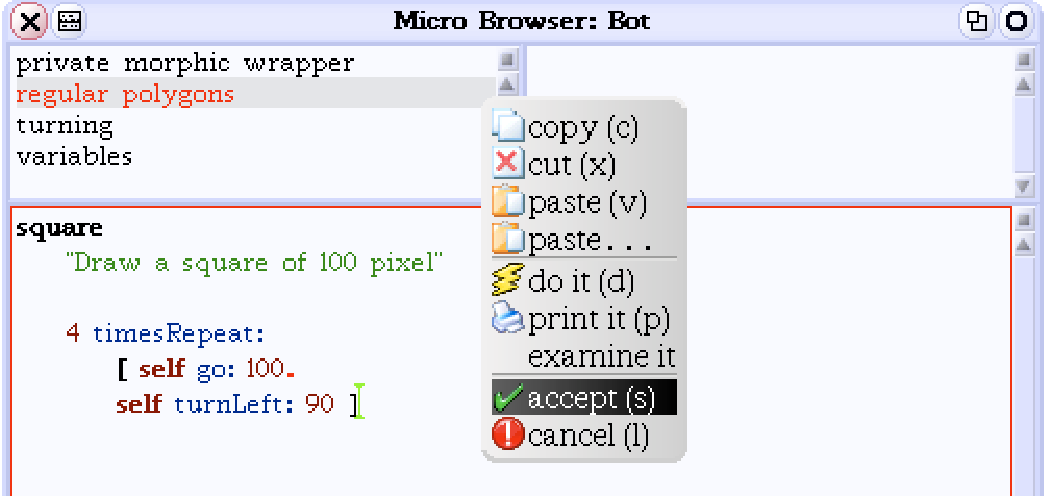
\includegraphics[width=10cm]{tbFive}} 
\caption{You have typed the method \ct{square} and now you should compile it using the code editor menu.\label{fig:firstMethod}}
\end{figure}

\paragraph{2. Compiling the method.} As shown by Figure~\ref{fig:compileMethod}, click to bring the menu  of the code editor and select the option \menu{Accept}.
This compiles the method \ie transform its definition into a representation that a computer can understand and execute. A new method named \ct{square} appears in the method list.  Note that if you made mistake while typing the method, \sq will report errors as we already discussed.

If you define correctly the method, you should be able to compile it, the browser reflects the fact that the compilation is done and that robots can now understand messages with the new method by showing the method name in the method category list (see Figure~\ref{fig:methodskeleton}).


%	\begin{figure}
%	\centerline{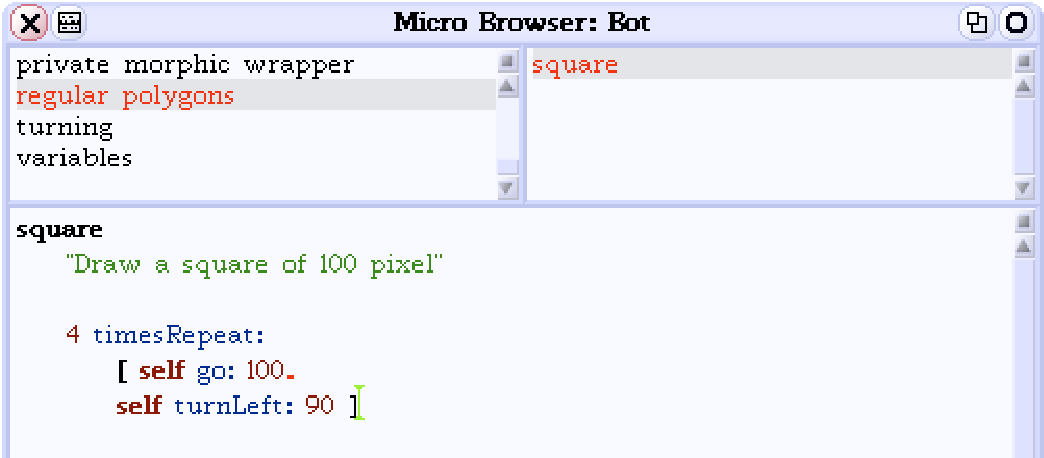
\includegraphics[width=15cm]{tbSix}} 
%	\caption{You have typed the method and compile the method \ct{square} 
%	now the browser reflects the fact that robot can understand messages with the 
%	new method.\label{fig:compileMethod}}
%	\end{figure}

\paragraph{3. Testing the method!} You do not have finished yet because 
the method you type may be wrong so you should test it.  Execute the
\scriptref{src:againSquareMethod}.

At this point you should realize that a method can be reused several times as demonstrated by \scriptref{src:againSquareMethod}.  Note that this fact this is not new. 
You used that since the beginning of this book: messages such as \go, \turnLeft and so on, are implemented as methods, just like the method \ct{square}. 

%%%%%%%%%%%%%%%%%%%%%%%%%%%%%%%%%%%%%%%%%%%%%%%%%%%
\section{What's in a Method?}
We asked you to type a method without much explanation. Now is the time to
analyze the structure of the method. A method is composed of a \emph{name}, an optional \emph{method comment} and a \emph{method body} (a sequence of messages) as shown by Figure~\ref{fig:methodskeleton}. To be exact, the method name can also contain parameters (See
chapter~\ref{ch:argumenting}), and the method body can contain also
definition of local variables using vertical bars \ct{|} and \ct{|}.

\begin{figure}
\centerline{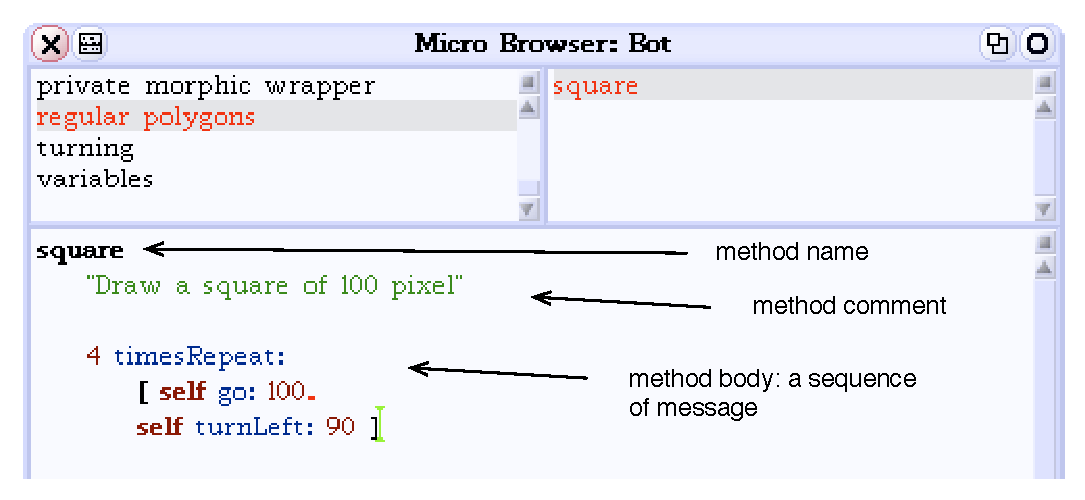
\includegraphics[width=15cm]{tbSixAnnotated}} 
\caption{A method is composed of a name, a method comment and a 
method body. \label{fig:methodskeleton}}
\end{figure}

\largecadre{A method name should always represent what the method does 
and not how it does it.}

\begin{description}
\item[Method Name.] 
A method name should always represent what the method does 
and not how it does it.  When you want to somebody to open a door, 
you do not explain him all the physic and mathematics involved. This is the 
same for method. 

Method names without parameters such as 
\ct{square} follow the same syntax as variable names. They are 
composed of alphanumerical characters and start with a
lowercase character. In our case the method name is \ct{square}.

\item[Method Comment.]
It consists of a text enclosed within a pair of double quotes
(\ct{"}). That text cannot contain any double quotes. However, a
comment can be as long as you like and can span itself
over several lines.  In general a comment explains the purpose and the 
effect of the method. It explains how the method can be used and not how 
the method is working. People who wants to know how the method is 
defined should read the method's body.

If the method name is explicit enough, the comment may be omitted.  
In our case the method comment is:
\begin{nalltt}
   "Draw a square of 100 pixel"
\end{nalltt}


\item[Method Body.] After the comment comes the method definition itself
\ie the sequence of messages that are executed in response to a message. In our case the 
method body is: 
\


\begin{nalltt}
   4 timesRepeat: 
         [ self go: 100.
         self turnLeft: 90 ]
\end{nalltt}
\end{description}
       
\largecadre{A method is a named sequence of messages. It is composed of
a name, a comment and a sequence of messages. Once a method is defined any robot can execute it in answer to a message with the same name.}       

\subsection{Script vs. Method: an Analysis}
If you compare the \methodref{mth:square} with the \scriptref{src:againSquare} you notice following differences:

\begin{itemize}
\item The line declaring the variable \caro is no longer here.
\item The line creating the robot has been suppressed.
\item In all other lines, the variable \caro is replaced by \self.
\end{itemize}

This should not be a surprise, since we already announced that a
method represents a sequence of messages which can be sent to
\emph{any} robot: the robot refered by the variable \caro is not necessarily the
receiver of the message \ct{square}. As we saw before \daly can also be a message receiver
of the message \ct{square}. Then, the message \ct{square} is sent to an \emph{existing}
robot. Thus, there is no need to create a robot since the one we want to send message to already
exists. This implies that while defining the method \ct{square}, we must have a way to refer to the object that will receive the message \ct{square}.  Indeed, we want to send to the object
receiving the message \ct{square} and only to this one, the sequence of
messages specified in the method body. Therefore we need a way to refer to the receiver of a message.  This is the purpose of \self. Inside a method, \self represents the object receiving a  message.

\paragraph{The \self variable.}
If you remember the discussion of Chapter~\ref{ch:variables}, a
variable is just a named placeholder for an object. In particular, we emphasized 
that the same variable could be used to point to different objects. 
In the case of a method, the variable \self points to the object that receives the message: when the message \ct{\caro\ square} is executed \self refers to the robot named \caro, when the
message \ct{\daly\ square} is executed \self refers to the robot named \daly.

To be complete, \self is a special variable because you cannot change its value. Only \sq can assign the value of \self. That's why \self does not have to be declared between vertical bars \ct{|}. Moreover, \self can only the used inside a method definition.

\largecadre{Inside a method the variable \ct{self} represents the 
object that receives the message. Therefore if messages have to be sent to the receiver, send messages to \self}


\paragraph{Method or Not: That's the Question.} At this stage you may be tempted to go back and convert all scripts you have been doing into methods. This is not advisable since not all scripts are worth themselves to be turned into a method. In general, one makes a method when a sequence of messages is sufficiently general to be used several times.

\section{Returning a Value}
A method can also return a value using the character up arrow \^\ also called \index{return} \index{caret} \index{returning a value} caret. Imagine that we want to have a method that returns the length that a robot should move in one movement. We can define the method \ct{maxLength} shown in~\ref{mth:maxLength}. Here the method is simply returning a number but we can return the result of any complex expression. 

\begin{method}\label{mth:maxLength}
maxLength 
   "returns the maximum length"

   ^ 100
\end{method}

By default every method returns the message receiver. The method~\ref{mth:squareEquivalent} is equivalent to the method \ct{square} defined previously. In fact at the end of every method there is an implicit expression \^ \self. However in the context of this book you do not have to worry about that. 

\begin{method}\label{mth:squareEquivalent}
squareEquivalent
   "Draw a square of 100 pixel size"

   4 timesRepeat: 
              [ self go: 100.
              self turnLeft: 90].
   ^ self
\end{method}

In the context of this book we will not use a lot this feature but this is important to know that a method always returns a value. 

\section{Pattern Drawing}\label{sec:newart}
Now it is time to practice. As you have seen, it is quite easy to transform a script into a method.  Many seasoned programmers use scripts to test ideas. When the feasibility of an idea has been proven in the form of a script, they move the code of the script into a method for later reuse. The next exercise trains you to do exactly this.

Let us consider the following script~\ref{src:artNouveau} which draws a geometric shape. 

\begin{scriptfig}{artNouveauScr}{A Simple Pattern}\label{src:artNouveau}
| \caro |
\caro := \Turtle new.
\caro go: 100 ;
        turnLeft: 90 ;
        go: 100 ;
        turnLeft: 90 ;
        go: 50 ;
        turnLeft: 90 ;
        go: 50 ;
        turnLeft: 90 ;
        go: 100 ;
        turnLeft: 90 ;
        go: 25 ;
        turnLeft: 90 ;
        go: 25 ;
        turnLeft: 90 ;
        go: 50
\end{scriptfig}

\begin{exonofig} \label{exo:artNouveau}
Create a method named \ct{pattern} which produces the drawing presented in Figure \scriptref{src:artNouveau}.
\end{exonofig}

We now can use this method in a script to draw a frame.

\begin{scriptfig}{artNouveauFourScr}{A Frame} 
\label{src:artNouveauFrame}
| \caro |
\caro := \Turtle new.
4 timesRepeat: [ \caro pattern ; go: 50 ]
\end{scriptfig}

At this point, some astute reader might ask: why don't we create a
method---named \ct{frame50}, for example---corresponding to
that of \scriptref{src:artNouveauFrame}. This is indeed possible
since \emph{any method created for robot can be reused
by another turtle method}. This is the topic of the next chapter. 

\begin{exonofig} \label{exo:artNouveauFrame50}
Create a method named \ct{frame50} which produces the picture produced by Script \ref{src:artNouveauFrame}. 
\end{exonofig}


\comment{
Nevertheless, let us convert one script, namely \scriptref{src:petal}
drawing a petal.

\begin{exonofig} \label{exo:mthPetal45}
Write a method named \ct{petal} corresponding to 
\scriptref{src:petal}. 
\end{exonofig}


In order to test whether the new method you created is correct,
you must write a simple script to test it, a script similar to
Script \ref{src:petal}. After this , try to use the method in a
more complex script.

\begin{exonofig} \label{exo:usePetal45}
Rewrite the script you have made for Exercise \ref{exo:flower} to
use the new method \ct{petal45}.
\end{exonofig}
}


\summa

\begin{enumerate}
\item A method is a named sequence of messages. It is composed of
a name, a comment and a sequence of messages. Once a method is defined any robot can execute it in answer to a message with the same name.

\item A method name should always represent what the method does 
and not how it does it. 

\item A new method for a robot is created using a \tb \ie a special 
editor to define methods. 

\item Inside a method the variable \ct{self} represents the 
object that receives the message. Therefore if messages have to be sent to the receiver, send messages to \self
\end{enumerate}


\subsection*{Glossary}
\begin{itemize}
\item Method categories. A method category is folder in which methods are sorted. It helps finding methods faster. 
\item Method. A method represents a sequence of messages that an object can execute. A method has a name. It is executed when an object receives a message having the same name. 
\item Browser. A browser is a special tool to view and edit methods. 
\item Comment. A comment is a piece of text delimited by "" that indicates the purpose of a method. 
\item \self. \self is a variable known predefined in \st that always represents the receiver of the message. 
\end{itemize}


\ifx\wholebook\relax\else\end{document}\fi
